\section{Neural networks}%
\label{sec:Neural networks}

A neural network is a machine learning model, that consists of a stack of layers. Neural networks are used to recognize patterns in data and be able to classify it. As an example in a self driving car a neural network could be used to recognize different real world objects, such as signs or pedestrians.

The way it works is by having some input data that can be used as a input to the network, and then be propageted through each layer. Propagation means that the data travel from one layer to the next and the layer's operation is applied to the network. \autoref{fig:example_nn} shows  a representation of a neural network with a couple of layers. In the example the white bar is a layer. The layer applies some operation to the input of the layer. Where the input of the layer is coming from the arrow that points to the layer. The input to the network is a vector $\bm{x}$ and the output of the network is a vector $\bm{y}$.

\begin{figure}
    \centering
    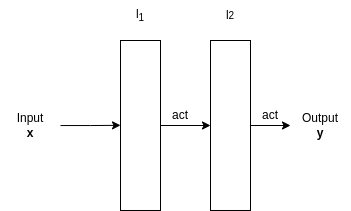
\includegraphics[width=0.7\textwidth]{assets/nn-simple-example.png}
    \caption{A simple neural network with 2 layers. \texttt{act} means an activation function is applied}
    \label{fig:example_nn}
\end{figure}

In \autoref{sub:network_training} it will be shown how a network can be trained to recognize patterns and be able to classify. A network can be trained with the help of a loss function, loss functions are functions that calculates how far from the correct output the network is.
% \autoref{fig:nn_out} shows the output probabilities   
When data is propagated through the network to the output, the network puts a probability on each output, the output that has the highest probability is what the network predicts as the classification.
The actual training aims to try to minimize the loss function, which makes it a problem of gradient descent, this will be described more in \autoref{sub:network_training}.

\subsection{Fully connected layer}%
\label{sub:Fully connected layer}

The fully connected layer is also known as a dense layer or a linear layer.
The fully connected layer can be used in deep learning after multiple convolutional layers, which will be discussed in \autoref{sub:nn_conv}.
Multiple fully connected layers can be stacked to create a multilayer perceptron. A multilayer perceptron can be used for classifying data that is linearly seperable \cite{perceptron}.

The layer consists of $M$ input neurons and $N$ output neurons. A neuron in this example is just a place to store a value.
The layer also consists of $M\times N$ synapses.
\autoref{fig:linear_example} shows an example representation of a fully connected layer. Each input neuron is connected to each output neuron with a synapse represented by a line. And \autoref{fig:neural_network} shows a generalization of the fully connected layer.

\begin{figure}
    \centering
    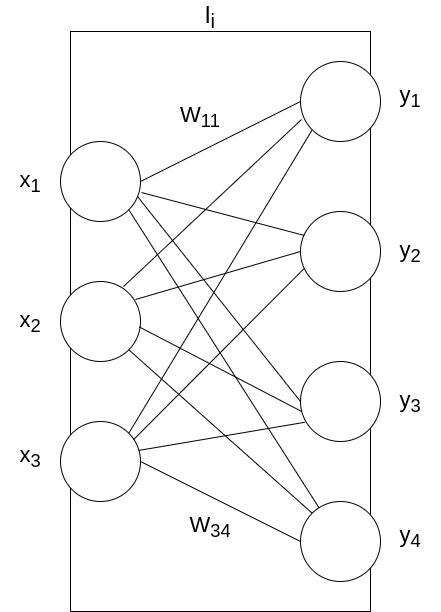
\includegraphics[width=0.5\textwidth]{assets/linear-layer-example.png}
    \caption{An illustration of a fully connected layer with 3 input neurons and 4 output neurons. The white bar in the background should illustrate that we are looking closer at a layer from \autoref{fig:example_nn}. (Only two weights are labeled here, but each line represents a weight in $\bm{W}$)}
    \label{fig:linear_example}
\end{figure}

The fully connected layers's input can be represented as a vector $\bm{x}$ and the output can also be represented as a vector $\bm{y}$.

\begin{figure}
    \centering
    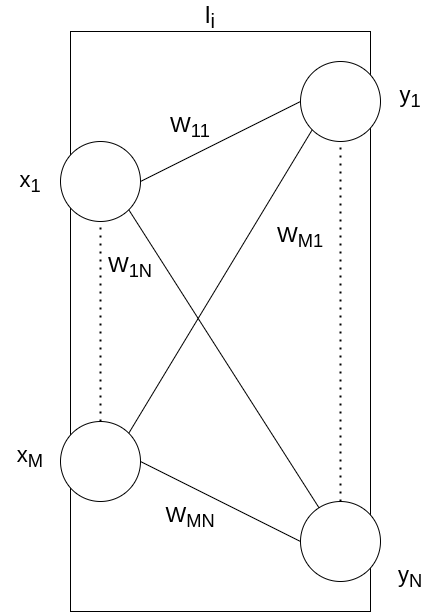
\includegraphics[width=0.5\textwidth]{assets/linear-layer.png}
    \caption{An illustration of a fully connected layer, where the dotted lines means there might be more values in between.}
    \label{fig:neural_network}
\end{figure}


The synapses works by having a weight which is multiplied to the value from the input when the value is propagated through the layer.
The weights of the synapses can be represented as a matrix $\bm{W}$, which will now be referred to as the weights.
The weight $w_{ij}$ corresponds to the weight between input $i$ and output $j$.
Where $i = 1, ..., M$ and $j = 1, ..., N$.

\autoref{fig:linear_propagation} shows what happens when input is propagated to an output neuron. When data is propagated through the layer, it moves from the input neuron through a synapse, where it is multiplied by the weight and then each value that ends in that output is summed together.

\begin{figure}
    \centering
    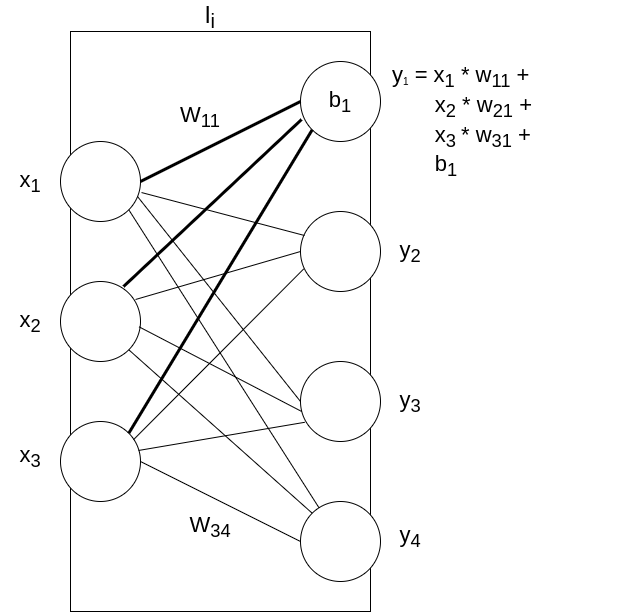
\includegraphics[width=0.6\textwidth]{assets/linear-layer-linear-propagation.drawio.png}
    \caption{Forward propagation of a fully connected layer for a single output, where the bold lines are the ones that are being used.}
    \label{fig:linear_propagation}
\end{figure}

The following formula shows this without the bias.
$$y''_j = \sum_{i=0}^D w_{ji}x_i  $$
After this step, a bias should be added as shown in \autoref{fig:linear_propagation}, the bias is added such that the layer can fit better to the data during training.
The bias $\bm{b}$ can be represented as a vector with the same length as the output $\bm{y}$ of length $N$.

$$y'_j = b_j + \sum_{i=0}^D w_{ji}x_i$$

The vector $\bm{y'}$ can thus be represented as a matrix-vector multiplication and adding the bias vector

$$\bm{y'} = \bm{b} + \bm{W}\bm{x}$$

At last, each output should apply an activation function $\bm{\sigma}$, activation functions are described in \autoref{sub:Activation functions}.
After applying the activation function $\bm{y}$ becomes
$$\bm{y} = \bm{\sigma} \left(\bm{y}'\right)$$

\subsection{Activation functions}%
\label{sub:Activation functions}

Activation functions have an important role in neural networks, since they can introduce non-linearity. This is important when training the network, because it can help the network converge toward a minima.
The activation function has it's name because it can tell if a neuron should "activate" or not. Consider the sigmoid function, when the input is less than 0 the output is close to $0$, and when it is greater than 0 it is close to 1. So the neuron can be called activated if the output of the neuron is close to 1.
Some common activation functions can be seen in \autoref{tab:activation}.

\begin{table}[H]
\centering
\begin{tabular}{|c|c|}\hline
\textbf{Function} & $\bm{\sigma}$ \\\hline
tanh     & $\frac{e^x - e^{-y'}}{e^x + e^{-y'}}$ \\\hline
ReLU     & $max(0, y')$ \\\hline
sigmoid  & $\frac{1}{1+e^{-y'}}$ \\\hline
softmax  & $\frac{e^{y'}}{\sum^K_{k=1} e^{y'_k}}$ \\\hline
\end{tabular}
\caption{A list of common activation functions.}
\label{tab:activation}
\end{table}
ReLU and softmax are the ones used in ResNet and seems to be the more popular choice, since it seems that these functions make the network converge faster during training.

\subsection{Convolutional layer}%
\label{sub:nn_conv}

\guillemotleft A convolutional neural network, or CNN, is a deep learning neural network designed for processing structured arrays of data such as images \guillemotright \cite{conv_article}.

A convolutional layer might take a three dimensional input, which corresponds to an image. Where the first dimension is the different channels, this could be different colors, such as red, green and blue. The next two dimensions is the actual image.

The goal of a convolutional layer is to detect certain features, in the given input data. The network will be able to detect more and more complex features depending on how many convolutional layers the network has.

\autoref{fig:conv_input_and_kernel} shows an example input dataset $\bm{X}$ and an example kernel\footnote{The kernel may also be called a filter in other sources.} $\bm{K}$.
\autoref{fig:conv_operation} shows an example of the convolutional operation, with a single channel. It could in fact have multiple channels which would then be added to the output, still with a single kernel that has the same number of channels as the input. The output will only have a single channel.
The kernel should have the same number of dimensions as the input data, but the size of the kernel should be less than or equal to the image, this can also be seen on \autoref{fig:conv_input_and_kernel}.

\begin{figure}
    \centering
    \hfill
    \subfloat[][An example for a $3 \times 3$ input to a convolutional layer]{$\begin{bmatrix}
        X_{11} & X_{12} & X_{13} \\
        X_{21} & X_{22} & X_{23} \\
        X_{31} & X_{32} & X_{33} 
    \end{bmatrix}$}
    \hfill
    \subfloat[][An example for a $2\times 2$ kernel]{$\begin{bmatrix}
        K_{11} & K_{12} \\
        K_{21} & K_{22}
    \end{bmatrix}$}
    \hfill
    \null
    \caption{An example for an input and a kernel to be used in a convolutional layer}
    \label{fig:conv_input_and_kernel}
\end{figure}


The convolutional operation works by taking the dotproduct of the kernel with a slice of the input. It is not really possible to take the dotproduct of two matrices, so it is assumed that they are flattened to vectors.  This is done for each channel with the same slice, adding it all together in the output. Then adding a bias and applying the activation function. This is repeated for a new slice until the the end of the input is reached.

\begin{figure}
    \centering
    $$\begin{bmatrix}
        \color{red} X_{11} & \color{red} X_{12} & X_{13} \\
        \color{red} X_{21} & \color{red} X_{22} & X_{23} \\
        X_{31} & X_{32} & X_{33} 
    \end{bmatrix} \otimes K \Rightarrow \begin{bmatrix}
        \color{red} X_{11} K_{11} + X_{12} K_{12} + X_{21} K_{21} + X_{22} K_{22} & \\
         &
    \end{bmatrix}$$\\
    $$\begin{bmatrix}
        X_{11} & \color{red} X_{12} & \color{red} X_{13} \\
        X_{21} & \color{red} X_{22} & \color{red} X_{23} \\
        X_{31} & X_{32} & X_{33} 
    \end{bmatrix} \otimes K \Rightarrow \begin{bmatrix}
         Y''_{11} &\color{red} X_{12} K_{12} + X_{13} K_{13} + X_{22} K_{22} + X_{23} K_{23} \\
         &
    \end{bmatrix}$$\\
    $$\begin{bmatrix}
        X_{11} & X_{12} & X_{13} \\
        \color{red} X_{21} & \color{red} X_{22} & X_{23} \\
        \color{red} X_{31} & \color{red} X_{32} & X_{33}
    \end{bmatrix} \otimes K \Rightarrow \begin{bmatrix}
        Y''_{11} & Y''_{12} \\
        \color{red} X_{21} K_{21} + X_{22} K_{22} + X_{31} K_{31} + X_{32} K_{32} & 
    \end{bmatrix}$$\\
    $$\begin{bmatrix}
        X_{11} & X_{12} & X_{13} \\
        X_{21} & \color{red} X_{22} & \color{red} X_{23} \\
        X_{31} & \color{red} X_{32} & \color{red} X_{33}
    \end{bmatrix} \otimes K \Rightarrow \begin{bmatrix}
         Y''_{11} & Y''_{12} \\
         Y''_{21} & \color{red} X_{22} K_{22} + X_{23} K_{23} + X_{32} K_{32} + X_{33} K_{33}
    \end{bmatrix}$$\\
    \caption{A visualization of the convolutional layer operation. The red numbers on the left are the input values that are currently in the window. The red number on the right is the result of the dotproduct of the window and the kernel.}
    \label{fig:conv_operation}
\end{figure}

\begin{figure}
    \centering
    $$\begin{bmatrix}
        \color{red} X_{11} & \color{red} X_{12} & X_{13} & X_{14} \\
        \color{red} X_{21} & \color{red} X_{22} & X_{23} & X_{24} \\
        X_{31} & X_{32} & X_{33} & X_{34}
    \end{bmatrix} \otimes K \Rightarrow ...$$\\
    $$\begin{bmatrix}
        X_{11} & X_{12} & \color{red} X_{13} & \color{red} X_{14} \\
        X_{21} & X_{22} & \color{red} X_{23} & \color{red} X_{24} \\
        X_{31} & X_{32} & X_{33} & X_{34}
    \end{bmatrix} \otimes K \Rightarrow ...$$\\
    \caption{Based on \autoref{fig:conv_operation}, but with an extra column on $X$ and a stride of 2 ($s_x = 2$, $s_y=2$). As it can be seen the values in the bottom of $X$ is never used in this example.}
    \label{fig:conv_operation_with_stride}
\end{figure}

The operation can end up with multiple output channels, there will be one output channel per kernel in the layer.

\autoref{fig:conv_operation_with_stride} shows how the stride can affect the output. In simple terms the stride describes how many steps there should be between each slice to be used.

To put it as a formula for the 2 dimensional image,
let $\bm{X}$ be the input,
$\bm{Y}$ be the output.
$b$ the bias.
$C_{in}$ the number of input channels.
$\bm{K}$ the kernel.
$k_x$ and $k_y$ the size of the kernel and $s_x$ and $s_y$ be the stride which the kernel is moving through the image.

$$Y_{ij} = b + \sum^{C_{in}}_{c = 1} \sum^{i \cdot s_x + k_x}_{i_2 = i \cdot s_x} \sum^{j \cdot s_y + k_y}_{j_2 = j \cdot s_y} X_{ci_2j_2} K_{ci_2j_2} $$

Where $i$ is the index in the first image dimension, $j$ is the index in the second image dimension.

$i$ and $j$ are in the following ranges

$$i = 1, ..., \left\lfloor\frac{n_x - k_x}{s_x}\right\rfloor + 1$$
$$j = 1, ..., \left\lfloor\frac{n_y - k_y}{s_y}\right\rfloor + 1$$

Where $n_x$ and $n_y$ are the image dimensions.

This means the dimensions of $\bm{Y}$ is

$$\left(\frac{n_x - k_x}{s_x} + 1\right) \times \left(\frac{n_y - k_y}{s_y} + 1\right) $$

\subsection{Maxpooling layer}

The maxpooling layer is used for downsampling and is often used in convolutional neural networks. The idea is that it accumulates features from feature maps generated by convolutional layers. Max pooling is used in order to avoid overfitting during training, since too many parameters might lead to overfitting \cite{maxpool_article}.

\autoref{fig:max_pool} shows how the max pooling layer partitions the input with different colors for each partition. The max pooling layer outputs the maximum value in each partition.

\begin{figure}[htpb]
    \centering
    $$\begin{bmatrix}
        \color{red}1 & \color{red} 2 & \color{green} 3 & \color{green} 4 \\
        \color{red}8 & \color{red}9 & \color{green}10 & \color{green}11 \\
        \color{blue}7 & \color{blue}1 & \color{magenta}2 & \color{magenta}6 \\
        \color{blue}2 & \color{blue}1 & \color{magenta}9 & \color{magenta}3
        \end{bmatrix} \Rightarrow \begin{bmatrix}
        \color{red}9 & \color{green}11 \\
        \color{blue}7 & \color{magenta}9
        \end{bmatrix}$$
    \caption{Illustration of a max pooling operation on a $4\times 4$ matrix with a $2\times 2$ window. The window will process the numbers of the same color and output the same color.}
    \label{fig:max_pool}
\end{figure}

In this example the first slice will be $[1, 2, 8, 9]$\footnote{the slice is flattened for easier readability}. Then the greatest number is $9$ which will be set in the output. This is repeated for the next slice and then repeated until every partition has been max pooled.

The maxpooling layer reduces the input, such that only the most important features are carried over to the next layer and thus reducing the number of operaitons needed for the nect layer.

\subsection{Loss functions}%
\label{sub:Loss functions}

To determine how close the network is at predicting something, a loss function can be used.
The loss function works by taking the output of the network and comparing it with the expected value or label.
This will be relevant in the following subsection (\autoref{sub:network_training}).

There are different loss functions that finds the loss in different ways. Some common loss functions can be seen in \autoref{tab:loss}

\begin{table}[ht]
\centering
\begin{tabular}{|c|c|}
\hline
\textbf{Loss function}  & \textbf{L(W)} \\ \hline
Cross entropy  & $-\sum^K_{k=1}(l_k\ ln\ y_k)$ \\ \hline
Mean squared error & $\frac{1}{K}\sum^K_{k=1}(y_k-l_k)^2$ \\ \hline
\end{tabular}
\caption{Some common loss functions, where $\bm{y}$ is the output of the network and $\bm{l}$ is the expected values or labels}
\label{tab:loss}
\end{table}

\subsection{Network training}%
\label{sub:network_training}

The goal of using a neural network is to make it correctly classify some input data.
To make the network classify input data correctly, the weights of each layer need to be changed in order to fit the input data and labels.
The network can be trained by using a loss function on the output of the network.

Let $L(\bm{X}, \bm{W}, \bm{Y})$ be a loss function over a network, where $\bm{X}$ be the input data to the network, $\bm{W}$ represents the weights of all layers and $\bm{Y}$ be the labels for the input data.
By taking the partial derivative of $L$ with respect to $\bm{W}$
$$\frac{\partial L}{\partial \bm{W}}$$
we can figure out how much $\bm{W}$ should be changed to move toward a minima for the loss function.

The process of trying to minimize $L$ can be done with gradient descent, where $\bm{X}$ and $\bm{Y}$ will be fixed values.

In \autoref{sec:autodiff} it will be discussed how to find the gradient or derivative of any function, which can be used for gradient descent.

\subsection{Exploding and vanishing gradients problem}

When using the backpropagation algorithm in a neural network, the gradient in some layers might be so small, that when updating the weights of the early layers, they will barely change. This problem is referred to as the vanishing gradients problem, as the gradients become so small that they almost vanish.
This problem makes it much harder to train a network since the weights might never reach the optimal value.
On the other hand the gradients might get so large that they move the weights way too much, such that the weights will never really hit an optimal value.
This problem can make the network significantly harder to train and maybe even impossible. This can, for example, make the application of vanilla SGD impossible \cite{exploding_gradients}.

This problem can be dealt with by using normalization layers which will be discussed in \autoref{sub:norm_layers}.


% There is no well-accepted metric for determining the presence of pathological exploding gradients \cite{exploding_gradients}.

\subsection{Batch normalizations layer}%
\label{sub:norm_layers}

% Motivation
\guillemotleft Batch Normalization allows us to use much higher learning rates and
be less careful about initialization. It also acts as a regularizer,
in some cases eliminating the need for Dropout \guillemotright \cite{batch_norm}.
Batch normalization can make training a network much faster, since the learning rate can be lower.
It also deals with the problem of exploding/vanishing gradients, which can help the network converge toward more optimal weights during training.

% How it works
% The idea of the Batch normalization layer is to normalize the the input of the layer, such that they are on the same scale.
% For example an input value might represent age which could be between 0 and 100, and another could be miles driven in a car which could be between 1000 and 100000 miles.
% These values 
One of the problems of training deep neural networks is that during training all layers' weights are updated simultaneously.
This is a problem since the gradient tells how much the weights should change while assuming that other layers do not change.
This causes a problem where each time the layers are updated it will have a new target, which might make the weights never settle during training.

The idea of a Batch normalization layer is to standardize input values to a layer.
The values are scaled such that it has a mean of zero and a standard deviation of one.
The standardization can be done by first calculating the mean and standard deviation of the input values, then using this to calculate the standardization.
$$\hat{x} = \frac{x - E[x]}{\sqrt{Var[x]}}$$
Where $\hat{x}$ is the standardized values for one dimension.
However the layer also have two new learnable parameters $\gamma$ and $\beta$.
These parameters are used to give the layer a new mean and standard deviation.
Where $\gamma$ scales the normalized values to give it a new standard deviation and $\beta$ shifts the values to a new mean.
The formula for the layer can then be represented as
$$y = \frac{x - E[x]}{\sqrt{Var[x]}} \cdot \gamma + \beta$$
% However in a Batch normalization layer the standardization can be done with the help of two new learnable parameter $\beta$ and $\gamma$, such that these values would not have to be calculated, but instead trained.


\subsection{Residual network (ResNet)}

\guillemotleft Deep convolutional neural networks have led to a series of breakthroughs for image classification\guillemotright \cite{resnet}.
To solve more and more complex tasks, deeper networks seems to be more accurate.
The problem is that the networks can not just get deeper and deeper since it seems that when a certain limit is reached accuracy is becoming saturated and after adding more layers accuracy seems to degrade.
An obstacle to this problem has also been the problem of vanishing/exploding gradients.
However ResNet is able to be accurate in considerably increased depth and have dealt with the problem of exploding/vanishing gradients by using normalization layers. ResNet also produces results substantially better than previous networks \cite{resnet}.

In this section there will be described which methods ResNet uses and how the model is structured.

% \subsubsection{Residual representation}

\subsubsection{Shortcut connections}

A shortcut connection is a connection that skips one or more layers and may have parameters that change the values.
\autoref{fig:shortcut_connection} shows an example of a shortcut connection that adds the input $\bm{x}$ value of the first layer to the output of the last layer.
Where $F(\bm{x})$ is the forward propagation of the block. The block in this case is just the two weight layers, but in general a block can have any number of layers.
In this case the shortcut connection is an identity mapping, meaning that the connection does not change the value of $\bm{x}$ during the shortcut connection.

\begin{figure}
    \centering
    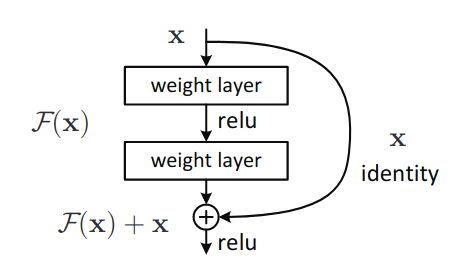
\includegraphics[width=0.55\textwidth]{assets/shortcut-connection.png}
    \caption{A shortcut connection represented by the arching arrow. $\mathcal{F}(\bm{x})$ is the function of applying $\bm{x}$ to the two layers. $\mathcal{F}(\bm{x}) + \bm{x}$ is the value after the shortcut connection. Source: \cite{resnet}}
    \label{fig:shortcut_connection}
\end{figure}

The benefit a shortcut connection is that it deals with the exploding/vanishing gradients problem, since it can allow the gradient to "flow" through to earlier layers, without exploding or vanishing in the same way.

\subsubsection{Deep residual learning}

Residual learning builds on the use of shortcut connections. 
This is done by having shortcuts with identity mapping for every few layers.
\guillemotleft The shortcut connections in Eqn.(1) introduce neither extra parameter nor computation complexity \guillemotright \cite{resnet}.
The only extra number of computation that is needed during residual learning is making an element-wise matrix-matrix addition, for every few layers.
The element-wise addition is computationally cheap, thus it can be a very good trade off if it means that the network might be trained faster and it might have better accuracy.

The dimensions of $\bm{x}$ and $\mathcal{F}(\bm{x})$ has to be equal, if they are not the data can be linearly projected by a matrix $\bm{W}_s$ to match the dimensions of $\bm{y} = \mathcal{F}(\bm{x}) + \bm{W}_s\bm{x}$.

\subsubsection{Netwok architecture}%

\autoref{fig:resnet} shows the two network archtectures: plain and residual.

\textbf{Plain network}: The convolutional layers mostly have $3 \times 3$ filters and follow two simple design rules:
\guillemotleft (i) for the same output
feature map size, the layers have the same number of filters; and
(ii) if the feature map size is halved, the number of filters is doubled so as to preserve the time complexity per layer
\guillemotright\cite{resnet}.
Whenever the data nis downsampled it is done by a convolutional layer with a stride of 2.
In the end the network has a fully connected layer with 1000 outputs.

\textbf{Residual network}: 
The residual network is based on the plain network, but uses shortcut connctions with identity mapping. However when the dimensions do not match for a shortcut connection (dotted line), the data is downsampled by using a $1 \times 1$ convolution with a stride of 2.
In the original implementation a batch normalization layer is used right after each convolution, which might help to deal with the exploding/vanishing gradients problem.

\begin{figure}
    \centering
    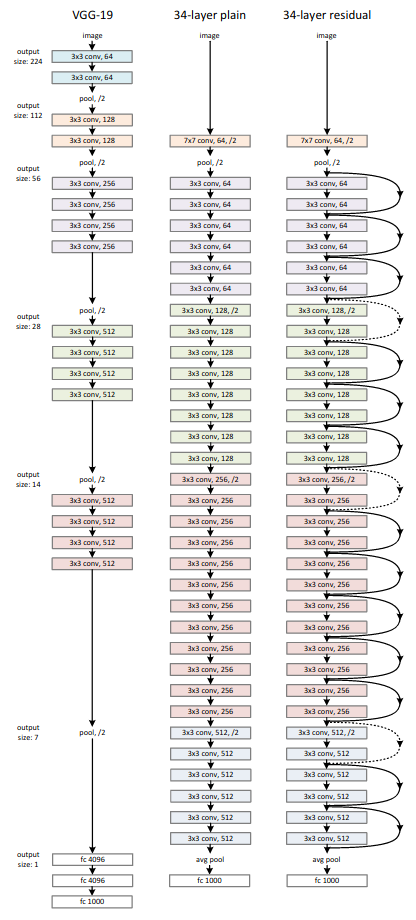
\includegraphics[scale=0.69]{assets/residual-net.png}
    \caption{The first part of each layer tells which type of layer it is, the second tells how many channels the layer uses, and the third tells if there is downsampling ($/2$). \textbf{middle}: 34-layer plain network. \textbf{right}: 34-layer residual network - based on plain, but with shortcut connections. The dotted lines represent a downsampling in the shortcut connection. Source: \cite{resnet}}
    \label{fig:resnet}
\end{figure}

